% Chapter 4

\chapter{Vorbereitung} % Main chapter title

\label{Chapter4} % For referencing the chapter elsewhere, use \ref{Chapter1}

%----------------------------------------------------------------------------------------

\section{Vorbereitung}
Bla

  \subsection{Extraktion von Named Entities}

  \subsection{Aufbereitung des Korpus}

  Als Textressource wurde das DECOW14X-Korpus (DE = Deutsch, COW = ``\textbf{CO}rpus from the \textbf{W}eb'') verwendet.
  Dieses Korpus von (\cite{schafer2012building})  besteht aus 21 Texten,
  die in den Jahren 2011 und 2014 von deutschsprachigen Internetseiten gecrawled und aufbereitet wurden. Dies beinhaltet
  PoS-Tagging, Chunking, Lemmatisierung, das Markieren von Eigennamen (Named Entities) und dem Hinzufügen von Metadaten.
  Die Sätze liegen darin im CoNLL-Format\footnote{Siehe http://ilk.uvt.nl/conll/ (zuletzt abgerufen am 11.04.16)} vor,
  wobei jedem Wort und dessen Annotationen eine ganze Zeile gewidmet ist,
  Stazgrenzen werden durch XML-Tags getrennt. Summa summarum enthält das Korpus 624.767.747 Sätze mit 11.660.894.000 Tokens.\\

  Für diese Arbeit wurden auf Basis der Ressource drei Version für das Training der Wortvektoren erstellt:
  \begin{itemize}
      \item Eine Datei mit den originalen Tokens durch Leerzeichen getrennt, je ein Satz pro Zeile.
      \item Eine Datei mit den lemmatisierten Tokens durch Leerzeichen getrennt, je ein Satz pro Zeile.
      \item Eine Datei mit dem lemmatisierten Tokens, sortiert nach den für jeden Satz geparsten Dependenzen, ein Satz pro Zeile.
  \end{itemize}
  Die Dependenzen wurden dabei mit dem Tool X erzeugt. [Blabla erläutern wenn Punkt erledigt.]


  \subsection{Training der Wortvektoren}

  Wortvektoren werden mithilfe des Tools \emph{word2vec} und zwei verschiedenen Modellen trainiert: Continuous-Bag-of-Words (CBOW)
  und Skip-Gram. Das CBOW-Model wurde zuerst von (\cite{mikolov2013efficient}) vorgestellt. Die Erklärung der Funktionsweise
  wird im nachfolgenden Teil recht klein gehalten, für eine ausführlichere und verständliche Ausführung wird beispielsweise
  die Arbeit von (\cite{rong2014word2vec}) empfohlen.\\

  Als Input fungieren ``One-Hot''-Vektoren, welche genau so viele Dimensionen wie Worte im Vokabular besitzen.
  Der Wert der Dimensionen entspricht $1$, wenn die Dimension der Stelle des aktuellen Wortes im Vokabular entspricht und
  ansonsten $0$. Die Modelle bestehen aus drei Schichten, namentlich \emph{Input}, \emph{Hidden} und \emph{Output}.
  Input und Output besitzen die Dimensionalität von $V$ ($V$ steht eigentlich für $\|\textsc{V}\|$, wird der Übersicht halber
  aber im Folgenden stellvertrentend dafür verwendet), Hidden die von $N$.\\

  \begin{figure}[h]
    \centering
    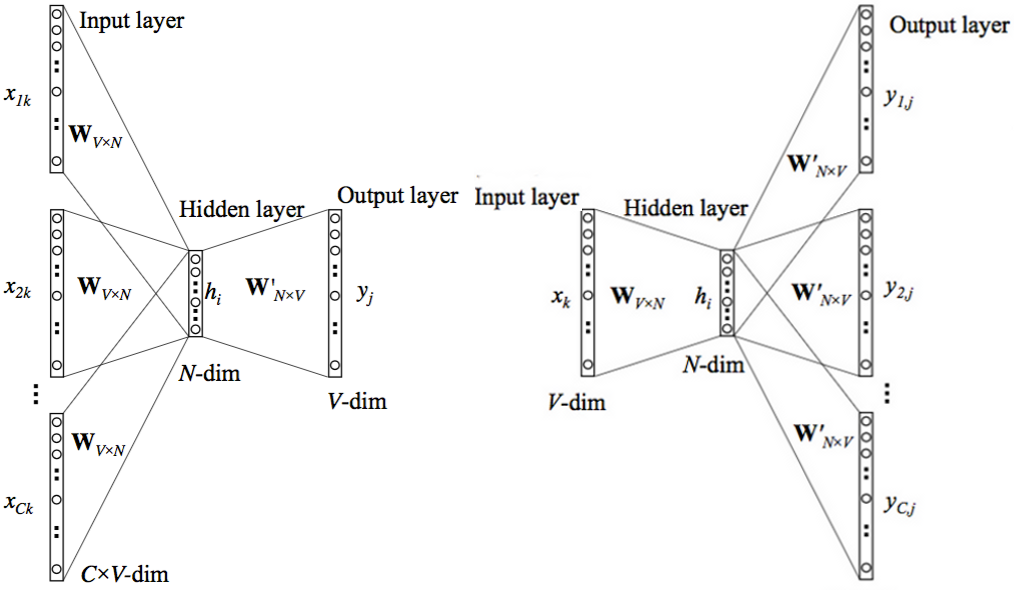
\includegraphics[width=1.1\textwidth]{../img/cbowskip.png}
    \caption[Gegenüberstellung von Skip-Gram und CBOW]{Gegenüberstellung der beiden Trainingsmethoden CBOW (links)
    und Skip-Gram (rechts). CBOW versucht die Wahrscheinlichkeit eines Wortes gegeben seines Kontexts zu trainieren,
    Skip-Gram die Wahrscheinlichkeit eines Kontextes gegeben eines Wortes.}
  \end{figure}

  Zwischen Input und Hidden liegt die Gewichtsmatrix $W$ und zwischen Hidden und Output die Matrix $W'$.
  CBOW versucht, die Wahrscheinlichkeit eines Wortes gegeben eines Kontextes
  der Größe $C$ zu maximieren (Kontext bezieht sich in diesem Fall auf die Summe der rechts und links vom Eingabewort stehenden
  Wörter). Unsere Verlustfunktion, deren Wert es dabei zu minimieren gilt, besteht darin in der negativen logarithmischen
  Wahrscheinlichkeit eines Wortes gegeben seines Kontextes:

  \begin{equation}
    E = - log\ p(w_O | w_{I,1}, \ldots, w_{I,C})
  \end{equation}

  Beim Skip-gram-Modell verhält sich das Ganze genau umgekehrt, es wird versucht, den Kontext gegeben eines Eingabewortes
  vorherzusagen:

  \begin{equation}
    E = - log\ p(w_{I,1}, \ldots, w_O)
  \end{equation}

  In beiden Fällen wird daraufhin überprüft, ob die Vorhersage mit den tatsächlichen Daten übereinstimmt und die Abweichung
  errechnet, mit der dann die Parameter der Gewichtsmatrizen $W$ und $W'$ rekursiv angepasst werden, um zukünftige Prognosen
  zu verbessen, wofür der \emph{Backpropagation}-Algorithmus verwendet wird. Die Wortvektoren, die dann nach dem Abarbeiten aller Trainingsdaten resultieren, sind dann die Zeilen von
  $W'$, wobei die \emph{i}-te Zeile der Matrix dem Wortvektor des Wortes mit dem Index \emph{i} im Vokabular entspricht.\\
  Eigentlich erfordert das Training eine aufwendige Berechnung über alle Wörter des Vokabels, was der Skalierbarkeit dieses
  Verfahrens entgegensteht. Der Aufwand kann allerdings durch Techniken wie \emph{Hierarchisches Softmax} oder, wie im
  Falle von \verb|word2vec|, \emph{Negativem Sampling} von $O(V)$ auf $O(log\ V)$ reduziert werden. Bei letzterem
  werden ``schlechte'' Beispiele zum Training hinzugezogen, woher sich auch der Name des Verfahrens ableitet.\\

  Dependenzgrammatiken untersuchen die Abhängigkeiten zwischen Wörtern eines Satzes und fügen diese in eine Dependenzstruktur ein.
  Anders als in der Phrasenstrukturgrammatik entsteht dabei kein Syntaxbaum mit Knoten. Worte stehen in Abhängigkeitsverhältnissen,
  wobei das das die Dependenz verursachende Wort alt \emph{Regens}, das davon abhängige als \emph{Dependenz} bezeichnet wird.\\
  (\citeauthor{levy2014dependency}) machen sich dies zunutze, um den Kontext beim Training von Wortvektoren neu zu definieren:
  Er besteht nun nicht mehr als den umgebenden Wörtern im Satz, sondern aus den Depenzen: Für ein Word $w$ mit den Modifizierern
  $m_1, \ldots m_k$ und den Kopf $h$ besteht der Kontext nun aus $(m_1, lbl_1), \ldots (m_k, lbl_k), (h, lbl_h^{-1})$, wobei
  $lbl$ stellvertretend für eine Dependenzrelation steht, ein $-1$ im Exponenten zeigt das Inverse einer solchen Relation an.
  Ein Beispiel dafür ist in Abb. X zu sehen.\\

  \begin{figure}[h]
      \centering
      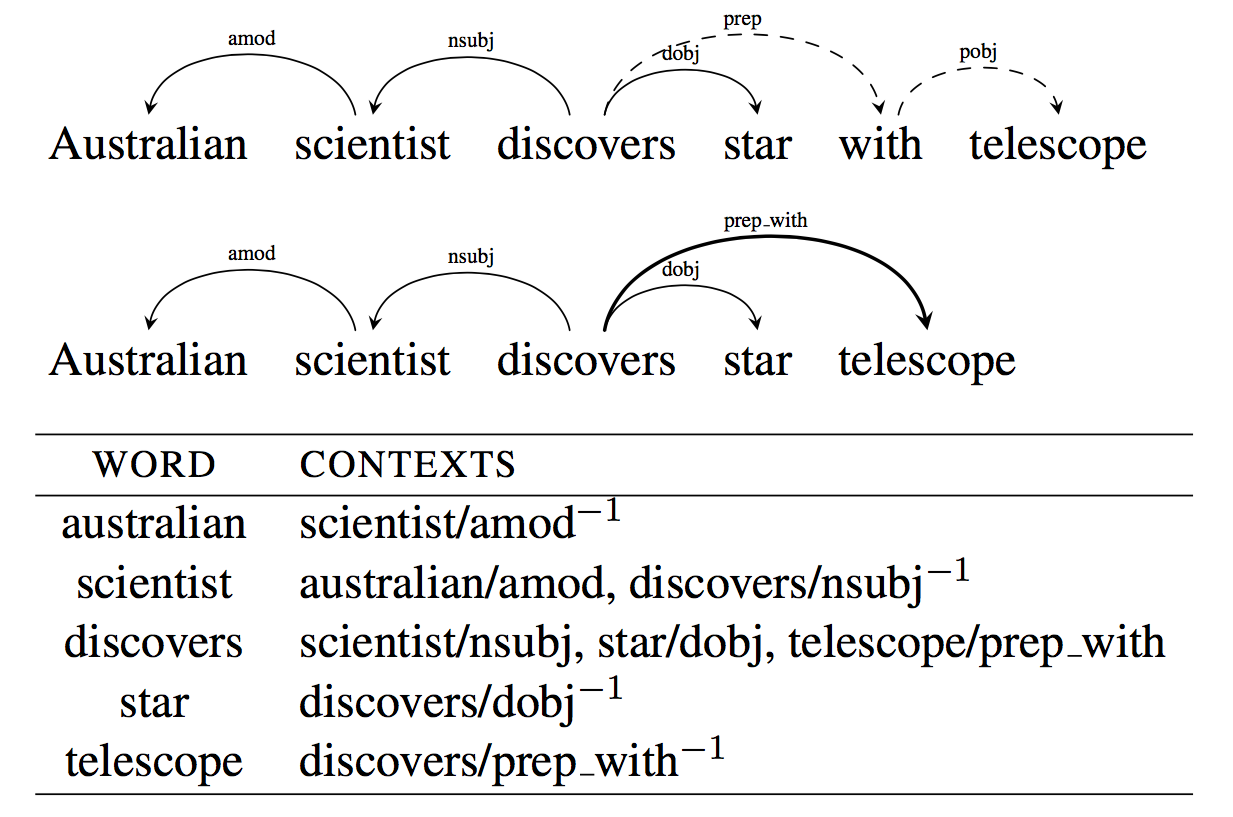
\includegraphics[scale=0.2]{../img/depend_ex.png}
      \caption[Erstellung von Dependenzkontexten beim Wortvektortraining]{Beispiel der Erstellung von Wortkontexten aus Dependenzen.
      Dependenzen mit Präposition werden zu einer Abhängigkeit zusammengefasst. \textbf{Oben}: Dependenzstruktur.
      \textbf{Unten}: Extrahierte Kontexte.}
  \end{figure}

  Zum Training der Vektoren wurde das C-Tool \emph{Word2Vec} von (\citeauthor{mikolov2013efficient}) verwendet. Als Eingabe
  benötigt es eine Textressource, die einen Satz pro Zeile enthält, Tokens durch Leerzeichen getrennt und gibt die Wortvektoren
  entweder einem einfach Text- oder Binärformat aus.\\
  Das Tool lässt zudem dem Nutzer offen, einige Parameter zu verändern. Jene, die in dieser Arbeit berücksichtigt wurden, sollen
  dabei näher erläutert werden:
  \begin{itemize}
    \item \verb|-sample|\\Die Wahrscheinlichkeit, mit der hochfrequente Worte
    \item \verb|-cbow|\\Bestimmt, welche Trainingsmethode verwendet wird ($0\ \hat{=}$ Skip-gram, $1\ \hat{=}$ Continuous-Bag-of-Words)
    \item \verb|-negative|\\Anzahl von negativen Beispielen beim Training.
  \end{itemize}

  Zwar bietet das Tool auch noch andere Parameter, jedoch soll aufgrund mit der Empfehlungen in (\citeauthor{levy2015improving}), in
  der eine große Anzahl von Konfigurationen ausprobiert wurde, im Rahmen dieser Arbeit nur mit den oben genannten Werten experimentiert werden.
